\section{Group -- Daylighting}\label{group-daylighting}

Daylighting can be invoked in EnergyPlus primarily by the use of the objects: \textbf{\hyperref[daylightingcontrols-000]{Daylighting:Controls}} and \textbf{\hyperref[daylightingreferencepoint-000]{Daylighting:ReferencePoint}}. Other objects related to daylighting are \textbf{Daylighting:DElight:ComplexFenestration}, \textbf{\hyperref[outputilluminancemap]{Output:IlluminanceMap}}, and \textbf{\hyperref[outputcontrolilluminancemapstyle]{OutputControl:IlluminanceMap:Style}}.  These are described in the following object descriptions.

\begin{callout}
  Note that two different methodologies are used in the \hyperref[daylightingcontrols-000]{Daylighting:Controls} object (SplitFlux and DElight) and may be intermixed in a single IDF but may not be used in the same zone.
\end{callout}

\subsection{Daylighting:Controls}\label{daylightingcontrols-000}

When this object is used, daylighting illuminance levels are calculated and then used to determine how much the electric lighting can be reduced. The daylight illuminance level in a zone depends on many factors, including sky condition; sun position; calculation point; location, size, and glass transmittance of windows; window shading devices; and reflectance of interior surfaces. Reduction of electric lighting depends on daylight illuminance level, illuminance set point, fraction of zone controlled and type of lighting control. Two different methods of computing the daylighting illuminance and subsequent lighting reduction called SplitFlux and DElight. After the object description below is are sections that describe the two methodologies in more detail.

\subsubsection{Inputs}\label{inputs-009}

\paragraph{Field: Name}\label{field-name-001}

The name of the Daylighting:Controls object.

\paragraph{Field: Zone or Space Name}\label{daylightingcontrols-field-zone-name}

The name of the \hyperref[zone]{Zone} or \hyperref[space]{Space} to which the following daylighting-related input applies. If a zone name is specified, the zone must lie completely within a single solar enclosure.

\paragraph{Field: Daylighting Method}\label{field-daylighting-method}

The Daylighting Method field can be set to either of the following: SplitFlux or DElight. Different Zones can have different settings in the same file but in a single zone only one method should be used at a time. Guidelines for using the SplitFlux method and additional details on the DElight method are shown in following sections.

\paragraph{Field: Availability Schedule Name}\label{field-availability-schedule-name-002}

This alpha field is optional and may be used to define the name of a schedule that denotes whether or not the control is available to operate during a given time period. If the schedule value is greater than zero, then the controls will be available to operate for that time period.~ If the schedule value is zero or less, then the controls will not be available. If this field is left blank, the controls will be always available. For example, this can be useful for scheduling the daylighting controls off during design days so that the daylighting controls do not affect lighting power during sizing.

\paragraph{Field: Lighting Control Type}\label{field-lighting-control-type}

The type of overhead electric lighting control. All reference points specified are assumed to have this type of control.

For Lighting Control Type set to Continuous, the overhead lights dim continuously and linearly from (maximum electric power, maximum light output) to (minimum electric power, minimum light output) as the daylight illuminance increases. The lights stay on at the minimum point with further increase in the daylight illuminance.

For Lighting Control Type set to Stepped, the electric power input and light output vary in discrete, equally spaced steps. The number of steps is given by Number of Steps (Excluding Off) of Stepped Control. For example, if Number of Steps = 3 and Illuminance Setpoint = 600, then the following table shows the fraction of the lights that are on vs. daylight illuminance.

% table 18
\begin{longtable}[c]{@{}ll@{}}
\caption{Example of a Stepped Lighting Control System with Three Steps \label{table:stepped-lighting-control-example}} \tabularnewline
\toprule
Daylight illuminance & Fraction of lights that are on \tabularnewline
\midrule
\endfirsthead

\caption[]{Example of a Stepped Lighting Control System with Three Steps} \tabularnewline
\toprule
Daylight illuminance & Fraction of lights that are on \tabularnewline
\midrule
\endhead

0-200 & 1.0 \tabularnewline
200-400 & 2/3 \tabularnewline
400-600 & 1/3 \tabularnewline
600 and above & 0.0 \tabularnewline
\bottomrule
\end{longtable}

Lighting Control Type set to ContinuousOff is the same similar to Lighting Control Type set to Continuous except that the lights switch off completely when the minimum dimming point is reached.

\paragraph{Field: Minimum Input Power Fraction for Continuous Dimming Control}\label{field-minimum-input-power-fraction-for-continuous-dimming-control}

For Lighting Control Type set to Continuous, the lowest power the lighting system can dim down to, expressed as a fraction of maximum input power (see figure, below). For Lighting Control Type set to ContinuousOff, this is the power fraction reached just before the lights switch off completely.

\begin{figure}[hbtp] % fig 54
\centering
\includegraphics[width=0.9\textwidth, height=0.9\textheight, keepaspectratio=true]{media/image096.png}
\caption{Illustration of continuous dimming relationship \protect \label{fig:illustration-of-continuous-dimming}}
\end{figure}

The figure shows the relationship between electric light output and electrical input.

\paragraph{Field: Minimum Light Output Fraction for Continuous Dimming Control}\label{field-minimum-light-output-fraction-for-continuous-dimming-control}

For Lighting Control Type set to Continuous, the lowest lighting output the lighting system can dim down to, expressed as a fraction of maximum light output (see figure). This is the fractional light output that the system produces at minimum input power. For Lighting Control Type set to ContinuousOff, this is the light output fraction reached just before the lights switch off completely.

\paragraph{Field: Number of Stepped Control Steps}\label{field-number-of-stepped-control-steps}

The number of steps, excluding off, in a stepped lighting control system (see figure, below). Required and must be \textgreater{}0 if Lighting Control Type is set to Stepped. The steps are assumed to be equally spaced.

\begin{figure}[hbtp] % fig 55
\centering
\includegraphics[width=0.9\textwidth, height=0.9\textheight, keepaspectratio=true]{media/image097.png}
\caption{Stepped lighting control with Number of Steps = 3. \protect \label{fig:stepped-lighting-control-with-number-of-steps}}
\end{figure}

\paragraph{Field: Probability Lighting will be Reset When Needed in Manual Stepped Control}\label{field-probability-lighting-will-be-reset-when-needed-in-manual-stepped-control}

May be specified if a stepped lighting control system (Lighting Control Type set to Stepped) is manually operated, such as in a simple, one-step (on-off) system. Gives the probability the occupants of a daylit zone will set the electric lights to the correct level to obtain the required illuminance. The rest of the time the lights are assumed to be set one step too high. For example, consider an on-off lighting system (Number of Steps = 1) with a set point of 600 lux and 0.7 reset probability. Then, when daylighting exceeds 600 lux, the electric lights will be off 70\% of the time and on 30\% of the time.

\paragraph{Field: Glare Calculation Daylighting Reference Point Name}\label{field-glare-calculation-daylighting-reference-point-name}

The \hyperref[daylightingreferencepoint-000]{Daylighting:ReferencePoint} name should be specified that is used for determining the glare. Only one reference point is used to calculate the glare. This input is only used in when the Daylighting Method is set to SplitFlux. This input is ignored when Daylighting Method is set to DElight.

\paragraph{Field: Glare Calculation Azimuth Angle of View Direction Clockwise from Zone y-Axis}\label{field-glare-calculation-azimuth-angle-of-view-direction-clockwise-from-zone-y-axis}

Daylight glare from a window depends on occupant view direction. It is highest when you look directly at a window and decreases as you look away from a window. This field specifies the view direction for calculating glare. It is the angle, measured clockwise in the horizontal plane, between the zone y-axis and the occupant view direction. This input is only used in when the Daylighting Method is set to SplitFlux. This input is ignored when Daylighting Method is set to DElight.

\paragraph{Field: Maximum Allowable Discomfort Glare Index}\label{field-maximum-allowable-discomfort-glare-index}

If a daylit zone has windows with shading devices (except exterior screens), the shades will be deployed if the daylight glare at \hyperref[daylightingreferencepoint-000]{Daylighting:ReferencePoint} specified in the Glare Calculation Daylighting Reference Point Name field exceeds the value of this field. To get this type of glare control you have to specify Trigger = Glare, GlareOrSolarOnWindow, GlareOrHorizontalSolar, GlareOrOutsideAirTemp, GlareOrZoneAirTemp or GlareOrZoneLoad in \hyperref[windowpropertyshadingcontrol]{WindowShadingControl} for one or more windows in the zone (see \hyperref[windowpropertyshadingcontrol]{WindowShadingControl}). This input is only used in when the Daylighting Method is set to SplitFlux. This input is ignored when Daylighting Method is set to DElight.

If a zone has two or more windows with glare control, the shading devices will be deployed one by one in the order in which the windows are input until the glare level at each reference point falls below Maximum Allowable Discomfort Glare Index or is as close as possible to it.

The following table gives recommended values of Maximum Allowable Discomfort Glare Index.

% table 19
\begin{longtable}[c]{@{}ll@{}}
\caption{Recommended Values of Maximum Allowable Discomfort Glare Index (DGI) \label{table:recommended-values-discomfort-glare-index}} \tabularnewline
\toprule
Activity or Zone Type & Maximum Allowable DGI \tabularnewline
\midrule
\endfirsthead

\caption[]{Recommended Values of Maximum Allowable Discomfort Glare Index (DGI)} \tabularnewline
\toprule
Activity or Zone Type & Maximum Allowable DGI \tabularnewline
\midrule
\endhead

Art Galleries & 16 \tabularnewline
Factories: Rough work & 28 \tabularnewline
Factories: Engine assembly & 26 \tabularnewline
Factories: Fine assembly & 24 \tabularnewline
Factories: Instrument assembly & 22 \tabularnewline
Hospital wards & 18 \tabularnewline
Laboratories & 22 \tabularnewline
Museums & 20 \tabularnewline
Offices & 22 \tabularnewline
School classrooms & 20 \tabularnewline
\bottomrule
\end{longtable}

\paragraph{Field: DElight Gridding Resolution}\label{field-gridding-resolution}

The maximum surface area for nodes in gridding (subdividing) all surfaces in the zone when Daylighting Method is set to DElight. All reflective and transmitting surfaces will be subdivided into approximately square nodes that do not exceed this maximum. Higher resolution subdivisions require greater calculation times, but generally produce more accurate results. This same gridding resolution is also used to subdivide any Complex Fenestration System surfaces. It is advisable to perform at least one simulation of new input using a small gridding resolution such as 0.1m2 to compare these results against simulation runs at lower resolution (i.e., higher maximum area nodal grids) to get a sense of possible levels of error. This input is only used in when the Daylighting Method is set to DElight. This input is ignored when Daylighting Method is set to SplitFlux.

\paragraph{Field Set (reference point name, fraction controlled, illuminance setpoint)}\label{field-set-daylightingcontrols}

This set of fields is used together and can be repeated an unlimited number of times to specify some of the name of the reference point, the fraction of the zone lighting controlled by that reference point and the illuminance setpoint that should be applied for daylighting control at that reference point.

\paragraph{Field: Daylighting Reference Point Name <x>}\label{field-daylighting-reference-point-name-x}

The \hyperref[daylightingreferencepoint-000]{Daylighting:ReferencePoint} name should be specified that is used for determining the daylighting control sensor location.

\paragraph{Field: Fraction of Lights Controlled by Reference Point <x>}\label{field-fraction-of-lights-controlled-by-reference-point-x}

The fraction of the zone or space's electric lighting is controlled by the daylight illuminance at the named \hyperref[daylightingreferencepoint-000]{Daylighting:ReferencePoint}. If the sum of the fractions are less than 1.0, the remaining portion is assumed to have no lighting control.

\paragraph{Field: Illuminance Setpoint at Reference Point <x>}\label{field-illuminance-setpoint-at-reference-point-x}

The desired lighting level (in lux) at the named \hyperref[daylightingreferencepoint-000]{Daylighting:ReferencePoint}. This is the lighting level that would be produced at this reference point at night if the overhead electric lighting were operating at full input power. Recommended values depend on type of activity; they may be found, for example, in the Lighting Handbook of the Illuminating Engineering Society of North America. A typical value for general office work (excluding computer terminals) is 500 lux.

\subsection{Daylighting:ReferencePoint}\label{daylightingreferencepoint-000}

This object is referenced by \hyperref[daylightingcontrols-000]{Daylighting:Controls} to identify the reference point coordinates for each sensor. The reference points in the zone are where horizontal daylighting illuminance will be calculated. It is assumed that the photocells that control the overhead electric lighting respond to the light levels at the specified coordinates. Reference points are given in coordinates specified in the \hyperref[globalgeometryrules]{GlobalGeometryRules} object Daylighting Reference Point CoordinateSystem field.

When the DElight Daylighting Method is used, there may be up to a maximum of 100 reference points for each zone. Each Reference Point that is input does NOT need to be included in the control of the electric lighting system within the zone. This is determined by the fraction of the zone controlled by each Reference Point, which can be input as 0. Note when the DElight Daylighting Method is used, that the sum of all Reference Point control fractions must equal 1 to obtain correct overall results.

It should also be noted that daylighting factors cannot be accurately calculated for reference points that are very close to a wall or window (less than 0.15 m or 6 inches). While an error is reported for a reference point that is too close to a window, no error message is generated when the user defines a point that is too close to a wall.

\subsubsection{Inputs}\label{inputs-010}

\paragraph{Field: Name}\label{field-name-002}

The name of the Daylighting:ReferencePoint object.

\paragraph{Field: Zone or Space Name}\label{daylightingreferencepoint-field-zone-name}

The name of the \hyperref[zone]{Zone} or \hyperref[space]{Space} in which the reference point is located.

\paragraph{Fields: (X,Y,Z) Coordinate of Reference Point}\label{fields-xyz-of-reference-point}

These three fields are the X, Y and Z values of the reference point in the coordinate system you specified for daylighting reference points in the \hyperref[globalgeometryrules]{GlobalGeometryRules} object. Figure~\ref{fig:example-showing-location-of-daylighting} shows an example using the relative coordinate (to zone) system. Z is typically at desk height (0.8 m).

\begin{figure}[hbtp] % fig 53
\centering
\includegraphics[width=0.9\textwidth, height=0.9\textheight, keepaspectratio=true]{media/image095.png}
\caption{Example showing location of daylighting reference points in the zone coordinate system (relative) of a rectangular zone with three windows. (a) Perspective view, (b) plan view, (c) elevation view. All dimensions are in meters. \protect \label{fig:example-showing-location-of-daylighting}}
\end{figure}




An IDF example:

\begin{lstlisting}

  Daylighting:Controls,
    West Zone_DaylCtrl,      !- Name
    West Zone,               !- Zone or Space Name
    SplitFlux,               !- Daylighting Method
    ,                        !- Availability Schedule Name
    Continuous,              !- Lighting Control Type
    0.3,                     !- Minimum Input Power Fraction for Continuous or ContinuousOff Dimming Control
    0.2,                     !- Minimum Light Output Fraction for Continuous or ContinuousOff Dimming Control
    ,                        !- Number of Stepped Control Steps
    1.0,                     !- Probability Lighting will be Reset When Needed in Manual Stepped Control
    West Zone_DaylRefPt1,    !- Glare Calculation Daylighting Reference Point Name
    180.0,                   !- Glare Calculation Azimuth Angle of View Direction Clockwise from Zone y-Axis {deg}
    20.0,                    !- Maximum Allowable Discomfort Glare Index
    ,                        !- DElight Gridding Resolution {m2}
    West Zone_DaylRefPt1,    !- Daylighting Reference Point 1 Name
    1.0,                     !- Fraction of Lights Controlled by Reference Point 1
    500.;                    !- Illuminance Setpoint at Reference Point 1 {lux}

  Daylighting:ReferencePoint,
    West Zone_DaylRefPt1,    !- Name
    West Zone,               !- Zone or Space Name
    3.048,                   !- X-Coordinate of Reference Point {m}
    3.048,                   !- Y-Coordinate of Reference Point {m}
    0.9;                     !- Z-Coordinate of Reference Point {m}

\end{lstlisting}

\subsection{Guidelines for Daylighting Modeling Using the SplitFlux Method)}\label{guidelines-for-daylighting-modeling-splitflux-method}

Following are some guidelines for preparing EnergyPlus input to model the effects of daylighting when using the SplitFlux method. Before studying these guidelines, however, you should read the description of each input field under \hyperref[daylightingcontrols-000]{Daylighting:Controls}, \hyperref[daylightingreferencepoint-000]{Daylighting:ReferencePoint}, and review the IDF example, above, and the sample daylighting input, PurchAirWithDaylighting.idf.

\subsubsection{Use of Window Multipliers}\label{use-of-window-multipliers}

If an exterior wall in a daylit enclosure has a number of identical windows, the windows should be entered separately rather than using a window multiplier (ref: \hyperref[fenestrationsurfacedetailed]{FenestrationSurface:Detailed}). Using a multiplier would give an incorrect illuminance calculation since individual windows would not be positioned correctly on the wall.

\subsubsection{Use of Zone Multipliers}\label{use-of-zone-multipliers}

A zone multiplier should not be used on a daylit zone if the windows in the zone are shadowed by exterior obstructions like trees or neighboring buildings, or by obstructions caused by other parts of building. The reason for this is that the shadowing on the windows of the multiplied zone may be different from zone to zone depending on exactly how the shadows fall on the zones. However, a zone multiplier may be used on a daylit zone if the shadowing is by overhangs, fins and/or window setback.

\subsubsection{Thermal Zoning for Daylighting}\label{thermal-zoning-for-daylighting}

To correctly calculate both direct and inter-reflected daylight illuminance you should try to model a thermal zone consisting of several similar rooms separated by interior walls as a representative room with a zone multiplier (ref: Zone). An example of this is shown in Figure~\ref{fig:for-daylighting-purposes-the-thermal-zone}. Room-1 is the representative room, with a zone multiplier = 4.

Interior walls IW-1, IW-2 and IW-3 should be treated as adiabatic, i.e., they should have Outside Boundary Condition = Surface and Outside Boundary Condition Object = IW-1, IW-2, or IW-3, respectively (ref: \hyperref[buildingsurfacedetailed]{BuildingSurface:Detailed}). Similarly, if the ceiling and floor of Room-1 are interior surfaces, they should be treated as adiabatic.

\begin{figure}[hbtp] % fig 56
\centering
\includegraphics[width=0.9\textwidth, height=0.9\textheight, keepaspectratio=true]{media/image098.png}
\caption{For daylighting purposes the thermal zone enclosed by the dashed boundary line should be modeled as a typical zone (Room-1) with a zone multiplier of 4. \protect \label{fig:for-daylighting-purposes-the-thermal-zone}}
\end{figure}

Sometimes a representative room cannot be found. Figure~\ref{fig:rooms-a-b-c-and-d-have-different-daylighting} shows a section of a building with four rooms having different daylighting characteristics because of different floor area, orientation and/or window size. In this case lumping the rooms into a single thermal zone would give nonsensical daylighting illuminance values because of the presence of the interior walls, which EnergyPlus ignores when calculating illuminance reaching a reference point directly from a window (i.e., without reflection). The solution in this case is to describe each room as a separate thermal zone with its own daylighting reference points, and input the interior walls because these will participate in the calculation of inter-reflected illuminance.

\begin{figure}[hbtp] % fig 57
\centering
\includegraphics[width=0.9\textwidth, height=0.9\textheight, keepaspectratio=true]{media/image099.png}
\caption{Rooms A, B, C and D have different daylighting characteristics. If lumped into a single thermal zone the daylighting calculation will be less accurate because the blockage of direct light by the interior walls between these rooms is modeled with some simplifications (see Interior Obstructions below). To get a good daylighting calculation each room should be input as a separate thermal zone. \protect \label{fig:rooms-a-b-c-and-d-have-different-daylighting}}
\end{figure}

\subsubsection{Multiple Lighting Zones}\label{multiple-lighting-zones}

The daylighting control calculation allows a thermal zone or space to be divided into multiple independently-controlled lighting zones. (See the fields: Daylighting Reference Point Name, Fraction of Lights Controlled by Reference Point, and Illuminance Setpoint at Reference Point.) An example is shown in Figure~\ref{fig:two-independently-controlled-lighting-zones}, where a relatively deep thermal zone has two lighting zones of equal area.

\begin{figure}[hbtp] % fig 58
\centering
\includegraphics[width=0.9\textwidth, height=0.9\textheight, keepaspectratio=true]{media/image100.png}
\caption{Two independently-controlled lighting zones, each with 50\% of the area of the thermal zone. \protect \label{fig:two-independently-controlled-lighting-zones}}
\end{figure}

\subsubsection{Fins, Overhangs and Other Exterior Obstructions}\label{fins-overhangs-and-other-exterior-obstructions}

The daylighting calculation accounts for the presence of exterior obstructions in determining the amount of light that strikes the windows. For daylighting purposes exterior obstructions fall into three categories:

\begin{itemize}
  \item
    Fins, overhangs, trees, neighboring buildings, etc., entered with the objects \hyperref[shadingzonedetailed-000]{Shading:Zone:Detailed}, \hyperref[shadingsitedetailed-shadingbuildingdetailed]{Shading:Site:Detailed}, or \hyperref[shadingsitedetailed-shadingbuildingdetailed]{Shading:Building:Detailed}.
  \item
    Building surfaces like walls and roofs (in an L-shaped building, for example).
  \item
    Surfaces associated with window setback.
\end{itemize}

Category (1) obstructions can have an associated solar transmittance schedule (see description of the field Transmittance Schedule Name for these shading surfaces). If this schedule is not specified, the surface is opaque (has zero transmittance).

The daylighting calculation takes the transmittance into account in determining, for example, how much light enters a window through a translucent awning. It is assumed that the solar and visible transmittance is the same and that the surfaces are non-diffusing, i.e., they do not change the direction of transmitted light. Ref:\hyperref[daylightingcontrols-000]{Daylighting:Controls}.

Category (2) and (3) surfaces are assumed to be opaque.

Surfaces in all three categories are assumed to be black, i.e., they do not reflect light, unless you set if ``Reflections'' option is chosen~ in the Building object. Then obstructions can reflect light, such as the top of an overhang reflecting light onto the window above. Ref: Building, Field: Solar Distribution (with reflections options).

\subsubsection{Interior Obstructions}\label{interior-obstructions}

The daylighting calculation accounts for the presence of interior obstructions that lie between a window and a reference point. Unlike exterior obstructions, which can be light transmitting, interior obstructions are assumed to be opaque. Interior obstructions can reduce or eliminate the light directly reaching the reference point through a window.

However, interior obstructions that are walls, ceilings or floors are reflecting so they~ contribute to the inter-reflected component of daylight illuminance as do the non-obstructing zone surfaces.

Interior obstructions can belong to the Shading object series. This type of obstruction is assumed to be non-reflecting so does not contribute to the inter-reflected component of daylight illuminance.

An example of an interior obstruction that is a wall in an L-shaped room is shown in Figure~\ref{fig:wall-a-or-wall-b-is-an-interior-obstruction}. Here, wall A (or, equivalently, Wall B) prevents light from directly getting to the Reference Point from the window.

\begin{figure}[hbtp] % fig 59
\centering
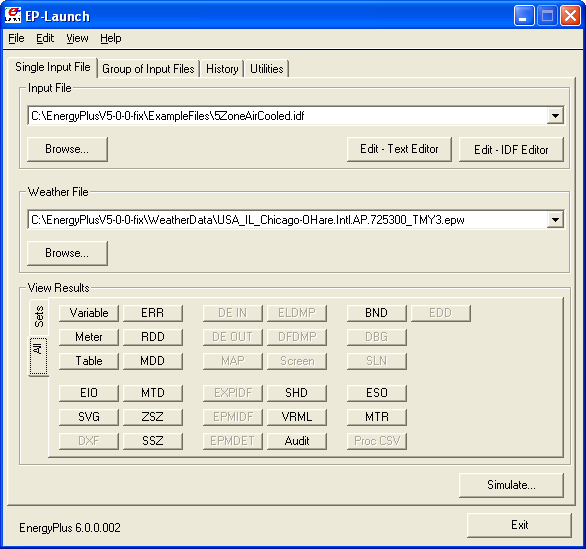
\includegraphics[width=0.9\textwidth, height=0.9\textheight, keepaspectratio=true]{media/image101.png}
\caption{Wall A (or Wall B) is an interior obstruction that prevents light from directly reaching the daylighting reference point from the window. \protect \label{fig:wall-a-or-wall-b-is-an-interior-obstruction}}
\end{figure}

\subsubsection{Double Façades: Daylighting through Interior Windows}\label{double-fauxe7ades-daylighting-through-interior-windows}

The \hyperref[daylightingcontrols-000]{Daylighting:Controls} method, with no additional user input,~ calculates the contribution of daylight that passes into a target zone through interior windows.\protect\hyperlink{ux5fftn1}{{[}1{]}} The origin of this daylight is exterior windows in adjacent zones that share interior windows with the target zone. This capability is aimed at daylighting through a \textbf{double façade} (also called ``double envelope'' or ``double skin.'')

This is illustrated in Figure~\ref{fig:vertical-section-through-a-double-faade}, which shows a double-façade buffer zone, Z0, with exterior windows EW1 and EW2. Z0 shares interior windows IW1, IW2 and IW3 with daylit occupied zones ZD1, ZD2 and ZD3, respectively (``daylit'' here means the zone has an associated \hyperref[daylightingcontrols-000]{Daylighting:Controls} object). The daylight illuminance at reference points RP1, RP2 and RP3 comes from the interior windows and has two main sources:

\begin{itemize}
  \item
    Daylight that passes through both an exterior window and an interior window in Z0 and reaches a reference point without reflection. This is called ``direct illuminance.''
  \item
    Daylight from Z0 that passes through an interior window and reaches a reference point by inter-reflection in the daylit zone. Because the program calculates this source from the interior solar distribution in Z0 it is recommended that the most accurate calculation of this distribution be made, which occurs if Solar Distribution = FullInteriorAndExterior in the Building object.
\end{itemize}

A third possible source is neglected because it is generally small in double-façade cases. This is daylight that is reflected from the surfaces of Z0, passes through an interior window and then reaches a reference point without inter-reflection in the daylit zone.

PurchAirWithDoubleFacadeDaylighting.idf is an input example of daylighting through an interior window.

\begin{figure}[hbtp] % fig 60
\centering
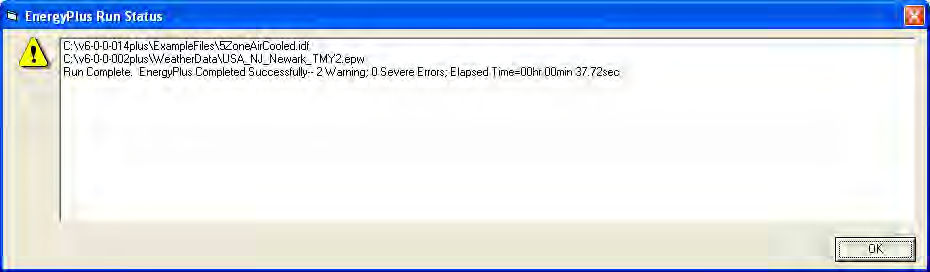
\includegraphics[width=0.9\textwidth, height=0.9\textheight, keepaspectratio=true]{media/image102.png}
\caption{Vertical section through a double-façade building showing daylighting through interior windows. The dashed lines show that (1) reference point RP1 receives direct light from exterior window EW1 via interior window IW1; (2) RP2 receives direct light from EW1 and EW2 via IW2; and (3) RP3 receives direct light from EW2 via IW3. \protect \label{fig:vertical-section-through-a-double-faade}}
\end{figure}

\subsubsection{Interior Window Daylighting Configurations that EnergyPlus Can Calculate}\label{interior-window-daylighting-configurations-that-energyplus-can-calculate}

Figure~\ref{fig:general-configuration-of-daylighting-through} shows schematically the general configuration of daylighting through interior windows that can be calculated with EnergyPlus. Here, daylit zone ZD has one or more interior windows that are adjacent to other zones, each of which has one or more exterior windows. ZD itself may or may not have exterior windows. If it does, than the daylight illuminance from its exterior and interior windows will be additive. The zones adjacent to ZD may or may not be daylit and may or may not have other interior windows that are not adjacent to ZD. (The program does not consider the illuminance in ZD from electric lighting in adjacent zones.)

\begin{figure}[hbtp] % fig 61
\centering
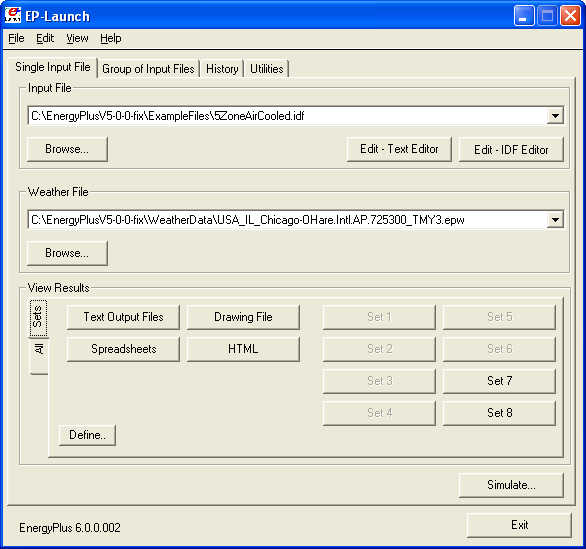
\includegraphics[width=0.9\textwidth, height=0.9\textheight, keepaspectratio=true]{media/image103.png}
\caption{General configuration of daylighting through interior windows that can be calculated with EnergyPlus. IW = interior window, EW = exterior window. \protect \label{fig:general-configuration-of-daylighting-through}}
\end{figure}

\subsubsection{Interior Window Daylighting Configurations that EnergyPlus Cannot Calculate}\label{interior-window-daylighting-configurations-that-energyplus-cannot-calculate}

Figure~\ref{fig:configuration-in-which-daylighting-of-zone-z} shows schematically a configuration of daylighting through interior windows that cannot be calculated with EnergyPlus. Here, zone Z has an interior window that is adjacent to zone Z1 which in turn has an interior window adjacent to zone Z2. However, the daylight from the exterior window in Z2 that enters Z after passing through Z1 is not calculated because Z2 is not adjacent to Z.

\begin{figure}[hbtp] % fig 62
\centering
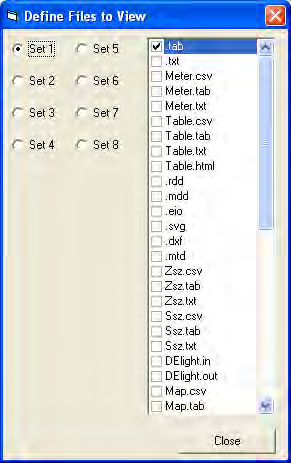
\includegraphics[width=0.9\textwidth, height=0.9\textheight, keepaspectratio=true]{media/image104.png}
\caption{Configuration in which daylighting of zone Z through its interior window  cannot be calculated with EnergyPlus. IW = interior window, EW = exterior window. \protect \label{fig:configuration-in-which-daylighting-of-zone-z}}
\end{figure}

\subsubsection{Restrictions on Shading Devices}\label{restrictions-on-shading-devices}

There are two restrictions on the use of exterior-window shading devices when a daylit zone has interior windows:

1)~~~If two daylit zones share an interior window, neither zone can have an exterior window whose shading device does glare control (i.e., the \hyperref[windowpropertyshadingcontrol]{WindowShadingControl} for the exterior window has Glare Control Is Active = Yes).

2)~~~If two daylit zones share an interior window, neither zone can have an exterior window with a \hyperref[windowpropertyshadingcontrol]{WindowShadingControl} that has Shading Control Type = MeetDaylightIlluminanceSetpoint.

\subsection{DElight Daylighting Method}\label{delight-daylighting-method}

The DElight method of analyzing daylighting in buildings is very similar to that used in the SplitFlux method and uses the same \hyperref[daylightingcontrols-000]{Daylighting:Controls} and \hyperref[daylightingreferencepoint-000]{Daylighting:ReferencePoint} objects but the Daylighting Method should be set to DElight. For each point in time, DElight calculates the interior daylighting illuminance at specified reference points and then determines how much the electric lighting can be reduced while still achieving a combined daylighting and electric lighting illuminance target. The daylight illuminance level in a zone depends on many factors, including exterior light sources; location, size, and visible light transmittance of simple and complex fenestration systems; reflectance of interior surfaces; and location of calculation reference points. The subsequent reduction of electric lighting depends on daylight illuminance level, illuminance set point, fraction of zone controlled, and type of lighting control.

There are two primary differences between the SplitFlux and DElight methods of calculating interior illuminance levels. The first is that DElight includes the capability of analyzing complex fenestration systems that include geometrically complicated shading systems (e.g., roof monitors) and/or optically complicated glazings (e.g., prismatic or holographic glass). The second key difference is that DElight uses a radiosity method to calculate the effects of light reflection inside a zone. These methods are discussed in more detail in the engineering documentation.

There are other important differences between the two methods. One is the inability of DElight to perform the type of dynamic shading controls possible using the SplitFlux method at each point in time during the thermal simulation (e.g., changes in electrochromic glazing transmittances and blind slat angles).  A second is the current lack of visual quality (e.g., glare) calculations performed by DElight. Third, the modeling of interior obstructions is different in the two methods. In the DElight method interior obstructions block interreflections but do not block the initial direct illuminance. In the SplitFlux method, interior obstructions block the initial direct illuminance but do not block interreflections. See the engineering documentation for more details. Fourth, when using DElight daylighting the presence of exterior shading surfaces such as overhangs is ignored.

Input for invoking the DElight method involves three object types: \textbf{\hyperref[daylightingcontrols-000]{Daylighting:Controls}}, \textbf{\hyperref[daylightingreferencepoint-000]{Daylighting:ReferencePoint}}, and \textbf{\hyperref[daylightingdelightcomplexfenestration]{Daylighting:DELight:ComplexFenestration}}.


\subsection{Daylighting:DELight:ComplexFenestration}\label{daylightingdelightcomplexfenestration}

Another input object that can only be used when the DElight Daylighting Method is used is  the Daylighting:DElight:ComplexFenestration object. The DElight daylighting analysis method can be applied to daylighting zones that contain only simple fenestration systems such as windows and skylights that are standard EnergyPlus sub-surfaces. In this situation, no Daylighting:DElight:ComplexFenestration object would be input.

In addition to analyzing simple fenestration systems, DElight includes the capability of analyzing complex fenestration systems such as geometrically complicated static shading systems (e.g., roof monitors) and/or optically complicated glazings (e.g., prismatic or holographic glass). This capability is based on characterizing these complex fenestration systems (CFS) using bi-directional transmittance distribution functions (BTDF). In general, BTDF data for a specific CFS must be either measured or simulated (e.g., using ray-tracing techniques) prior to employing DElight to analyze it within EnergyPlus. The current implementation of DElight CFS calculations within EnergyPlus supports two approaches to the input of BTDF, an analytical approach and a file-based approach. The details of inputting these two approaches are described below under the User Complex Fenestration Type field.

Two analytical CFS BTDF types are currently supported, window and light shelf. The file-based approach requires that a user has access to a data file containing raw BTDF data that DElight reads as additional input during its analysis calculations. BTDF data files are described separately since it is anticipated that individual EnergyPlus users will not create these data files themselves.

The methods related to characterizing and analyzing CFS using BTDF are still evolving. DElight is an early implementation of CFS analysis methods. These methods, and the input associated with them here, will likely change in the future.

\subsubsection{Inputs}\label{inputs-3-007}

\paragraph{Field: User Name}\label{field-user-name}

User name of the DElight daylighting Complex Fenestration to which the following input applies.

\paragraph{Field: Complex Fenestration Type}\label{field-complex-fenestration-type}

Type name of the DElight daylighting Complex Fenestration system to be analyzed. This type name must take one of the following two forms.


\begin{lstlisting}

BTDF^GEN^Analytical Type^Normal Visible Transmittance^Dispersion Angle

BTDF^FILE^Filename

\end{lstlisting}

The first form above is for supported analytical CFS types which currently include WINDOW and LIGHTSHELF. While these analytical types are relatively simple, they represent flexible ways to explore diffusing CFS systems and the impact of light shelves in redirecting light through an aperture. Each of these types also requires the visible transmittance of the CFS at normal incidence angle, and a dispersion angle (in degrees) that represents the ``spread'' of transmitted light. A small dispersion angle of 10 corresponds to clear glazing while a large angle of 90 corresponds to perfectly diffusing glazing. The ``\^{}'' symbol must be used as a delimiter between sub-fields within this Complex Fenestration type name string as shown in the IDF example for WINDOW below, and in the DElight sample input data files.

The second form above is for CFS types for which there is pre-measured or pre-simulated BTDF data. In this case the Filename sub-field must be a valid data file name that is associated with an existing BTDF dataset that DElight can use in its calculations.

\paragraph{Field: Building Surface Name}\label{field-building-surface-name}

The name of the heat transfer surface object instance hosting this Complex Fenestration, analogous to the Building Surface Name field for subsurfaces such as Windows. This must be a valid name that has been associated with a heat transfer surface contained in the same EnergyPlus input data file.

\paragraph{Field: Window Name}\label{field-window-name}

The name of the Window (ref: \hyperref[fenestrationsurfacedetailed]{FenestrationSurface:Detailed} object) instance that will be used to account for the geometry, and the solar/thermal gains/losses, of the Complex Fenestration system surface. This must be a valid name that has been associated with a Window contained in the same EnergyPlus input data file. The geometry for the Complex Fenestration is taken from the geometry input for this standard EnergyPlus subsurface, hence the term ``Doppelganger.''

Note that DElight only deals with the visible spectrum of light transmitted through a Complex Fenestration. To account for the solar/thermal influences of a Complex Fenestration, a geometrically coincident subsurface that will be accounted for by methods already within EnergyPlus must be defined in the input data file. This is an interim solution to the issue of accounting for solar/thermal influences that will likely change as techniques analogous to the daylighting analysis of BTDF are developed.

\paragraph{Field: Fenestration Rotation}\label{field-fenestration-rotation}

The in-plane counter-clockwise rotation angle between the Complex Fenestration optical reference direction and the base edge of the Doppelganger Surface geometry. The Complex Fenestration optical reference direction is the direction of the zero azimuth angle for the BDTF dataset. This Rotation angle will typically be zero when the Doppelganger surface is rectangular and its width edge is aligned with the Complex Fenestration optical reference direction.

An IDF example for an analytical WINDOW type CFS:

\begin{lstlisting}

Daylighting:DELight:ComplexFenestration,
      Window CFS,       !- DElight Complex Fenestration User Name
      BTDF^GEN^WINDOW^1.0^20.0,     !- Complex Fenestration Type
      ZN003:WALL001,  !- Complex Fenestration Host Surface
      Zn003:Wall001:Doppel001, !- Doppelganger Surface Name
      0.0;            !- Fenestration Rotation {deg}
\end{lstlisting}

\subsubsection{Outputs}\label{outputs-1-004}

The following daylighting-specific outputs are available for Daylighting:Controls:

\begin{itemize}
\item
  Zone,Average,Site Exterior Beam Normal Illuminance {[}lux{]}
\item
  Zone,Average,Site Exterior Horizontal Beam Illuminance {[}lux{]}
\item
  Zone,Average,Site Exterior Horizontal Sky Illuminance {[}lux{]}
\item
  Zone,Average,Site Beam Solar Radiation Luminous Efficacy {[}lum/W{]}
\item
  Zone,Average,Site Sky Diffuse Solar Radiation Luminous Efficacy {[}lum/W{]}
\item
  Zone,Average,Site Daylighting Model Sky Clearness {[]}
\item
  Zone,Average,Site Daylighting Model Sky Brightness {[]}
\item
  Surface,Average,Daylighting Window Reference Point <x> View Luminance {[}cd/m2{]}
\item
  Surface,Average,Daylighting Window Reference Point <x> Illuminance {[}lux{]}
\item
  Zone,Average,Daylighting Reference Point <x> Illuminance {[}lux{]}
\item
  Zone,Average,Daylighting Reference Point <x> Glare Index {[]}
\item
  Zone,Sum,Daylighting Reference Point <x> Glare Index Setpoint Exceeded Time {[}hr{]}
\item
  Zone,Sum,Daylighting Reference Point <x> Daylight Illuminance Setpoint Exceeded Time {[}hr{]}
\item
  Zone,Average,Daylighting Lighting Power Multiplier {[]}
\end{itemize}

\paragraph{Site Exterior Beam Normal Illuminance {[}lux{]}}\label{site-exterior-beam-normal-illuminance-lux}

Beam normal illuminance of the sun at the earth's surface, measured in lux (lumens/m\(^{2}\))

\paragraph{Site Exterior Horizontal Beam Illuminance {[}lux{]}}\label{site-exterior-horizontal-beam-illuminance-lux}

Beam illuminance on an unobstructed horizontal plane at the earth's surface. Equals ``Site Exterior Beam Normal Illuminance'' times sine of solar altitude.

\paragraph{Site Exterior Horizontal Sky Illuminance {[}lux{]}}\label{site-exterior-horizontal-sky-illuminance-lux}

Illuminance from sky solar radiation on an unobstructed horizontal plane at the earth's surface. The total exterior horizontal illuminance is the sum of ``Site Exterior Horizontal Beam Illuminance'' and ``Site Exterior Horizontal Sky Illuminance.''

\paragraph{Site Beam Solar Radiation Luminous Efficacy {[}lum/W{]}}\label{site-beam-solar-radiation-luminous-efficacy-lumw}

A measure of the visible light content of beam solar radiation; equal to the number of lumens per watt of beam solar radiation. Depends on atmospheric conditions (moisture, turbidity, cloudiness) and solar altitude.

\paragraph{Site Sky Diffuse Solar Radiation Luminous Efficacy {[}lum/W{]}}\label{site-sky-diffuse-solar-radiation-luminous-efficacy-lumw}

A measure of the visible light content of sky diffuse solar radiation; equal to the number of lumens per watt of sky diffuse solar radiation. Depends on atmospheric conditions (moisture, turbidity, cloudiness) and solar altitude.

\paragraph{Site Daylighting Model Sky Clearness {[]}}\label{site-daylighting-model-sky-clearness}

Clearness of sky. One of the factors used to determine sky type and luminous efficacy of solar radiation (see \emph{EnergyPlus Engineering Document}). Sky Clearness close to 1.0 corresponds to an overcast sky. Sky Clearness \textgreater{} 6 is a clear sky.

\paragraph{Site Daylighting Model Sky Brightness {[]}}\label{site-daylighting-model-sky-brightness}

Brightness of sky. One of the factors used to determine sky type and luminous efficacy of solar radiation (see \emph{EnergyPlus Engineering Document}).

\paragraph{Daylighting Window Reference Point <x> View Luminance {[}cd/m2{]}}\label{daylighting-window-reference-point-1-view-luminance-cdm2}

The area-averaged luminance of an exterior window as viewed from the first reference point in the daylit zone containing the window. In general, higher window luminance values are associated with higher daylight glare values. (Printed only for exterior windows in daylit zones without interior windows.)

\paragraph{Daylighting Window Reference Point <x> Illuminance {[}lux{]}}\label{daylighting-window-reference-point-1-illuminance-lux}

The contribution from a particular exterior window to the daylight illuminance at the first reference point in the daylit zone containing the window. (Not printed for exterior windows in daylit zones with interior windows.)

\paragraph{Daylighting Reference Point <x> Illuminance {[}lux{]}}\label{daylighting-reference-point-1-illuminance-lux}

The total daylight illuminance at the first reference point from all of the windows in a daylit zone.

\paragraph{Daylighting Reference Point <x> Glare Index {[]}}\label{daylighting-reference-point-1-glare-index}

The daylight glare index at the first reference point in a daylit zone.

\paragraph{Daylighting Reference Point <x> Glare Index Setpoint Exceeded Time {[}hr{]}}\label{daylighting-reference-point-1-glare-index-setpoint-exceeded-time-hr}

The number of hours when the calculated daylight glare index at the first reference point exceeds the glare index setpoint.

\paragraph{Daylighting Reference Point <x> Daylight Illuminance Setpoint Exceeded Time {[}hr{]}}\label{daylighting-reference-point-1-daylight-illuminance-setpoint-exceeded-time-hr}

The number of hours when the calculated daylight illuminance at the first reference point exceeds the daylight illuminance setpoint.

\paragraph{Daylighting Lighting Power Multiplier {[]}}\label{daylighting-lighting-power-multiplier-1}

The amount by which the overhead electric lighting power in a space or zone is multiplied due to usage of daylighting to dim or switch electric lights. For example, if the multiplier is M and the electric power without dimming is P, then the electric power with dimming is M*P. The multiplier varies from 0.0, which corresponds to maximum dimming (zero electric lighting), to 1.0, which corresponds to no dimming.

\subsection{Output:IlluminanceMap}\label{outputilluminancemap}

The Output:IlluminanceMap object expands on the reporting capabilities of the daylighting simulation. For any space or zone simulated with \hyperref[daylightingcontrols-000]{Daylighting:Controls}, the illuminance map can generate up to 2,500 points of additional daylighting illuminance values. The resulting map is output as a comma delimited text file that can be imported into a spreadsheet program for rapid visualization of the daylighting illuminance patterns in a space or zone. The values are produced on an hourly basis. The Z height of the map is constant (parallel to a flat floor). More than one illuminance map can be created for a space or zone. IlluminanceMap output is available only when SplitFlux daylighting method is selected in \hyperref[daylightingcontrols-000]{Daylighting:Controls} object.

When using the Output:IlluminanceMap object, the user should note the following:

\begin{itemize}
\item Daylighting factors cannot be accurately calculated for reference points that are very close to a wall or window (less than 0.15 m or 6 inches). An error is reported for a reference point that is too close to a window, but no error is reported for a point that is too close to a wall.
\item Since not all zones are rectangular, it is possible to have map points that are outside the zone. Any illuminance registered at these points is inaccurate and, additionally, a ``*'' marks these values for easy observance.
\end{itemize}

\subsubsection{Inputs}\label{inputs-4-006}

\paragraph{Field: Name}\label{field-name-2-007}

The name of the map object.

\paragraph{Field: Zone or Space Name}\label{field-zone-name-2-000}

Reference to a zone or space with \hyperref[daylightingcontrols-000]{Daylighting:Controls}. If a zone name is specified, all spaces in the zone must be within the same solar enclosure.

\paragraph{Field: Z Height}\label{field-z-height}

The height or elevation of the grid of daylighting points.  Coordinates may be world or relative as specified in the \hyperref[globalgeometryrules]{GlobalGeometryRules} object Daylighting Reference Point CoordinateSystem field. If a space name is specifice for this map, relative coodinates are relative to the origin of the zone that contains the space  (spaces do not have a separate origin).

\paragraph{Field: X Minimum Coordinate}\label{field-x-minimum-coordinate}

The minimum X coordinate boundary for the map.

\paragraph{Field: X Maximum Coordinate}\label{field-x-maximum-coordinate}

The maximum X coordinate boundary for the map.

\paragraph{Field: Number of X Grid Points}\label{field-number-of-x-grid-points}

The number of daylighting reference points in the X direction from the minimum to the maximum boundaries. The maximum number of points that can be generated is 2500 (Number of X Grid Points X Number of Y Grid Points).

\paragraph{Field: Y Minimum Coordinate}\label{field-y-minimum-coordinate}

The minimum Y coordinate boundary for the map.

\paragraph{Field: Y Maximum Coordinate}\label{field-y-maximum-coordinate}

The maximum Y coordinate boundary for the map.

\paragraph{Field: Number of Y Grid Points}\label{field-number-of-y-grid-points}

The number of daylighting reference points in the Y direction from the minimum to the maximum boundaries. The maximum number of points that can be generated is 2500 (Number of X Grid Points X Number of Y Grid Points).

\begin{lstlisting}

Output:IlluminanceMap,
    Daylit Map,      ! Map Name
    Daylit Zone,     ! Zone or Space Name
    0,               ! Z Height [m]
    0.1,             ! X Minimum Coordinate [m]
    4.9,             ! X Maximum Coordinate [m]
    10,              ! Number of X Grid Points
    0.1,             ! Y Minimum Coordinate [m]
    9.9,             ! Y Maximum Coordinate [m]
    10;              ! Number of Y grid Points
\end{lstlisting}

\subsection{OutputControl:IlluminanceMap:Style}\label{outputcontrolilluminancemapstyle}

This object specifies the ``style'' for the illuminance map output (described in the Output Details and Examples document). As described early in the document (see: EnergyPlus Output Processing), the user may select the ``style'' for the daylighting illuminance map output file (eplusmap.\textless{}ext\textgreater{}).

\subsubsection{Inputs}\label{inputs-5-006}

\paragraph{Field: Column Separator}\label{field-column-separator}

For this field, the desired separator for columns is entered. ``Comma'' creates comma separated fields/columns in the outputs (eplusmap.csv file is created). ``Tab'' creates tab separated fields/columns in the outputs (eplusmap.tab file is created). ``Fixed'' creates space separated fields/columns in the outputs (eplusmap.txt file is created) but these are not necessarily lined up for easy printing.

Note that both tab and comma separated files easily import into Excel\textsuperscript{TM} or other spreadsheet programs. The tab delimited files can also be viewed by text editors, word processing programs and easily converted to ``tables'' within those programs.

\subsection{Daylighting Devices}\label{daylighting-devices}

Daylighting devices work in conjunction with the \hyperref[daylightingcontrols-000]{Daylighting:Controls} object to simulate components that can improve daylighting in a zone.

Daylighting devices are also tightly integrated into the zone heat balance. The thermal effects of these devices are simulated with or without the use of a \hyperref[daylightingcontrols-000]{Daylighting:Controls} object.

There are two types of daylighting device in EnergyPlus:~ tubular daylighting devices and daylighting shelves.

\subsection{DaylightingDevice:Tubular}\label{daylightingdevicetubular}

Tubular daylighting devices (TDDs), also known as tubular skylights or light pipes, are used to bring natural exterior daylight into the hard-to-reach, interior spaces of a building.

TDDs consist of three components: a dome, a pipe, and a diffuser.

\begin{figure}[hbtp] % fig 66
\centering
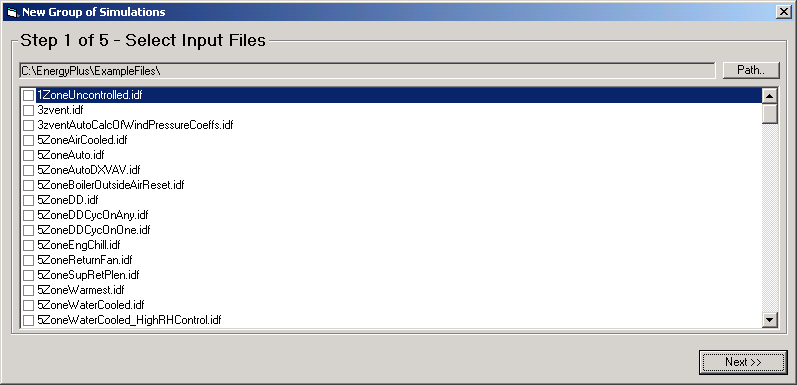
\includegraphics[width=0.9\textwidth, height=0.9\textheight, keepaspectratio=true]{media/image108.png}
\caption{Tubular daylighting device diagram. \protect \label{fig:tubular-daylighting-device-diagram.}}
\end{figure}

In EnergyPlus each of these components corresponds to an object in the input file.

The dome and diffuser are defined in the same way as windows using the \hyperref[fenestrationsurfacedetailed]{FenestrationSurface:Detailed} object. The \emph{Surface Type} field must be specified as TubularDaylightDome or TubularDaylightDiffuser accordingly.

The location and orientation of the dome surface affect the total amount of daylight collected.

The \emph{Base Surface} of the diffuser object determines to which zone the daylighting is delivered. The location and orientation of the diffuser surface affect the amount of daylight received at the \hyperref[daylightingcontrols-000]{Daylighting:Controls} reference points.

Although the object definition is the same as for a window, there are several restrictions on TubularDaylightDome and TubularDaylightDiffuser objects:

\begin{itemize}
\item
  Shading control devices are not allowed.
\item
  Frames and dividers are not allowed.
\item
  Multipliers must be 1.0.
\item
  Dome, diffuser, and pipe areas (as given by diameter) must be approximately equal.
\item
  Outside face environment objects are not allowed.
\item
  Dome and diffuser constructions cannot be more than one layer.
\end{itemize}

Since commercial TDDs are assumed to be cylindrical in shape, it is recommended that the circular areas of the actual dome and diffuser be approximated with a square of equivalent area for the TubularDaylightDome and TubularDaylightDiffuser objects. Although it is possible to use a triangular surface instead, a square is a much better geometric approximation of a circle.

Note that the TubularDaylightDome surface is allowed to have a different position and tilt from the roof base surface. If the actual TDD projects some height above the roof surface, the TubularDaylightDome coordinates should be located accordingly.

\begin{figure}[hbtp] % fig 67
\centering
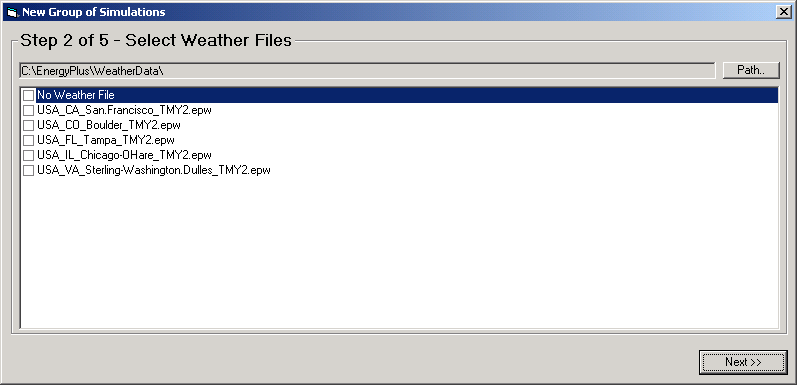
\includegraphics[width=0.9\textwidth, height=0.9\textheight, keepaspectratio=true]{media/image109.png}
\caption{Tubular daylighting device DXF output. \protect \label{fig:tubular-daylighting-device-dxf-output.}}
\end{figure}

The TubularDaylightDome surface automatically casts a shadow on the roof base surface. However, since the pipe is not represented by a surface, it will not cast a shadow. If this effect must be simulated, one or more SURFACE:SHADING objects can be used.

The dome and diffuser objects are connected by the DAYLIGHTING DEVICE:TUBULAR object:

\subsubsection{Inputs}\label{inputs-6-005}

\paragraph{Field: Name}\label{field-name-3-007}

The name of the TDD object.

\paragraph{Field: Dome Name}\label{field-dome-name}

Reference to a \hyperref[fenestrationsurfacedetailed]{FenestrationSurface:Detailed} object with \emph{Surface Type} TubularDaylightDome.

\paragraph{Field: Diffuser Name}\label{field-diffuser-name}

Reference to a \hyperref[fenestrationsurfacedetailed]{FenestrationSurface:Detailed} object with \emph{Surface Type} TubularDaylightDiffuser.

\paragraph{Field: Construction Name}\label{field-construction-name-001}

The construction of the TDD pipe. The visible and solar absorptance of the inside material layer determines the reflectivity of the inner mirrored surface of the TDD. This is very important for the overall transmittance of the TDD.

\paragraph{Field: Diameter}\label{field-diameter}

The diameter {[}m{]} of the TDD pipe. The area of the pipe must match the areas of the dome and diffuser.

\paragraph{Field: Total Length}\label{field-total-length}

The total length {[}m{]} of the TDD pipe between the dome and the diffuser, including the exterior part above the roof. The exterior length is determined internally by subtracting the transition zone lengths from the total length.

\paragraph{Field: Effective Thermal Resistance}\label{field-effective-thermal-resistance}

The effective thermal resistance {[}m\(^{2}\)-K/W{]}, i.e. R-value, of the TDD between the exterior dome surface and the interior diffuser surface.

\paragraph{Field: Transition Zone\textless{}\#\textgreater{}~ Name}\label{field-transition-zone-name}

Name of zone that the TDD pipe passes through before reaching the delivery zone.

\paragraph{Field: Transition Zone \textless{}\#\textgreater{} Length}\label{field-transition-zone-length}

Length of pipe {[}m{]} in the transition zone. This is used for determining heat gains due to solar absorbed by the pipe in each transition zone. The distribution of absorbed solar gains can be customized by adjusting the length of pipe in each transition zone.~~ The transition zone gain is proportional to the length of pipe in the zone. If no transition zones are specified, all solar absorbed by the pipe is lost to the exterior environment.

The \emph{Transition Zone Name} and \emph{Transition Zone Length} fields can be repeated for additional transition zones.

\begin{lstlisting}
DaylightingDevice:Tubular,
  Pipe1,                    !- Object Name
  Dome1,                    !- Dome Name
  Diffuser1,                !- Diffuser Name
  Reflective Aluminum,      !- Construction Name
  0.3556,                   !- Diameter [m] (approximately 14", a standard size)
  1.4,                      !- Total Length [m] (subtract zone lengths to get outdoor exposed length)
  0.28,                     !- Effective Thermal Resistance [m2-K/W] between TubularDaylightDome and TubularDaylightDiffuser
  Attic Zone,               !- Transition Zone 1 Name
  1.1;                      !- Transition Zone 1 Length [m]

FenestrationSurface:Detailed,
  Dome1,  !- Subsurface Name
  TubularDaylightDome,  !- Surface Type
  Clear Acrylic Dome,  !- Construction Name (only 1 layer allowed in construction)
  Attic Roof,  !- Base Surface Name
  ,  !- Outside Face Environment (not allowed for TubularDaylightDome)
  0.0,  !- VF to Ground
  ,  !- Window Shading Control (not allowed for TubularDaylightDome)
  ,  !- Frame/Divider Name (not allowed for TubularDaylightDome)
  1.0,  !- Multiplier (must be 1.0 for TubularDaylightDome)
  4,  !- Number of Vertices
  2.3425,  3.1575,  3.9,
  2.3425,  2.8425,  3.9,
  2.6575,  2.8425,  3.9,
  2.6575,  3.1575,  3.9;

FenestrationSurface:Detailed,
  Diffuser1,  !- Subsurface Name
  TubularDaylightDiffuser,  !- Surface Type
  Frosted Acrylic Diffuser,  !- Construction Name (only 1 layer allowed in construction)
  Daylit Zone Ceiling,  !- Base Surface Name
  ,  !- Outside Face Environment (not allowed for TubularDaylightDiffuser)
  0.0,  !- VF to Ground
  ,  !- Window Shading Control (not allowed for TubularDaylightDiffuser)
  ,  !- Frame/Divider Name (not allowed for TubularDaylightDiffuser)
  1.0,  !- Multiplier (must be 1.0 for TubularDaylightDiffuser)
  4,  !- Number of Vertices
  2.3425,  3.1575,  2.5,
  2.3425,  2.8425,  2.5,
  2.6575,  2.8425,  2.5,
  2.6575,  3.1575,  2.5;
\end{lstlisting}

\subsubsection{Outputs}\label{outputs-2-004}

\begin{itemize}
\item
  Zone,Average,Tubular Daylighting Device Transmitted Solar Radiation Rate {[}W{]}
\item
  Zone,Average,Tubular Daylighting Device Pipe Absorbed Solar Radiation Rate {[}W{]}
\item
  Zone,Average,Tubular Daylighting Device Heat Gain Rate {[}W{]}
\item
  Zone,Average,Tubular Daylighting Device Heat Loss Rate {[}W{]}
\item
  Zone,Average,Tubular Daylighting Device Beam Solar Transmittance {[]}
\item
  Zone,Average,Tubular Daylighting Device Beam Visible Transmittance {[]}
\item
  Zone,Average,Tubular Daylighting Device Diffuse Solar Transmittance {[]}
\item
  Zone,Average,Tubular Daylighting Device Diffuse Visible Transmittance {[]}
\end{itemize}

\paragraph{Tubular Daylighting Device Beam Solar Transmittance {[]}}\label{tubular-daylighting-device-beam-solar-transmittance}

This is the transmittance of beam solar radiation through the TDD.

\paragraph{Tubular Daylighting Device Beam Visible Transmittance {[]}}\label{tubular-daylighting-device-beam-visible-transmittance}

This is the transmittance of beam visible radiation, or daylight, through the TDD.

\paragraph{Tubular Daylighting Device Diffuse Solar Transmittance {[]}}\label{tubular-daylighting-device-diffuse-solar-transmittance}

This is the transmittance of diffuse solar radiation through the TDD.

\paragraph{Tubular Daylighting Device Diffuse Visible Transmittance {[]}}\label{tubular-daylighting-device-diffuse-visible-transmittance}

This is the transmittance of diffuse visible radiation, or daylight, through the TDD.

\paragraph{Tubular Daylighting Device Heat Gain Rate {[}W{]}}\label{tubular-daylighting-device-heat-gain-rate-w}

This is the rate of heat gain to the zone by the TDD, in Watts.

\paragraph{Tubular Daylighting Device Heat Loss Rate {[}W{]}}\label{tubular-daylighting-device-heat-loss-rate-w}

This is the rate of heat loss from the zone by the TDD, in Watts.

\paragraph{Tubular Daylighting Device Pipe Absorbed Solar Radiation Rate {[}W{]}}\label{tubular-daylighting-device-pipe-absorbed-solar-radiation-rate-w}

This is the rate at which solar radiation is absorbed by the pipe in the TDD, in Watts.

\paragraph{Tubular Daylighting Device Transmitted Solar Radiation Rate {[}W{]}}\label{tubular-daylighting-device-transmitted-solar-radiation-rate-w}

This is the rate at which solar radiation is transmitted by the TDD, in Watts.

In addition, several surface and window variables are also reported for the TubularDaylightDome and TubularDaylightDiffuser objects. For the TubularDaylightDome:

\begin{itemize}
\item
  Zone,Average,Surface Outside Face Sunlit Area {[}m2{]}
\item
  Zone,Average,Surface Outside Face Sunlit Fraction {[]}
\item
  Zone,Average,Surface Outside Face Incident Solar Radiation Rate per Area{[}W/m2{]}
\item
  Zone,Average,Surface Outside Face Incident Beam Solar Radiation Rate per Area{[}W/m2{]}
\item
  Zone,Average,Surface Outside Face Incident Sky Diffuse Solar Radiation Rate per Area{[}W/m2{]}
\item
  Zone,Average,Surface Outside Face Incident Ground Diffuse Solar Radiation Rate per Area{[}W/m2{]}
\item
  Zone,Average,Surface Outside Face Beam Solar Incident Angle Cosine Value{[]}
\item
  Zone,Average,Surface Window Transmitted Solar Radiation Rate {[}W{]}
\item
  Zone,Average,Surface Window Total Glazing Layers Absorbed Solar Radiation Rate {[}W{]}
\end{itemize}

For the TubularDaylightDiffuser:

\begin{itemize}
\item
  Zone,Average,Surface Outside Face Incident Solar Radiation Rate per Area{[}W/m2{]} \emph{(incident inside of pipe)}
\item
  Zone,Average,Surface Window Transmitted Solar Radiation Rate {[}W{]} \emph{(same as Tubular Daylighting Device Transmitted Solar Radiation Rate)}
\item
  Zone,Average,Surface Window Total Glazing Layers Absorbed Solar Radiation Rate {[}W{]}
\end{itemize}

\subsection{DaylightingDevice:Shelf}\label{daylightingdeviceshelf}

Daylighting shelves, or simply light shelves, are another device for bringing more daylight into a building. Installed as an accessory to a window, daylighting shelves work by reflecting exterior light onto the ceiling of a room. Daylighting shelves can have an inside shelf, an outside shelf, or both.

\begin{figure}[hbtp] % fig 68
\centering
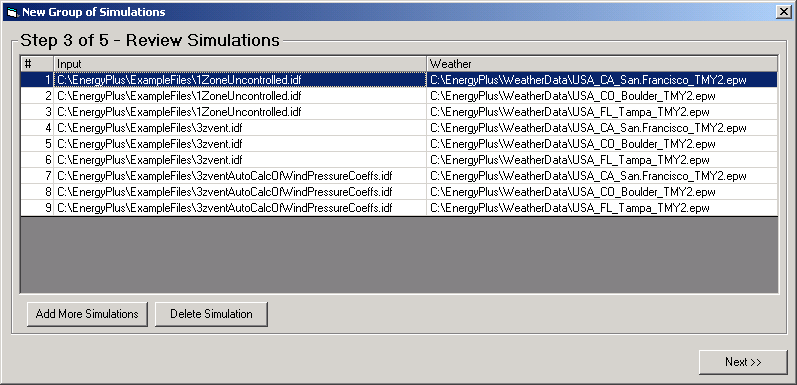
\includegraphics[width=0.9\textwidth, height=0.9\textheight, keepaspectratio=true]{media/image110.png}
\caption{Daylighting shelf diagram. \protect \label{fig:daylighting-shelf-diagram.}}
\end{figure}

The inside shelf redistributes light that would have entered the zone anyway. Instead of entering as a beam, all light is reflected onto the zone ceiling and is converted to diffuse shortwave radiation.

The outside shelf changes the amount of light entering the zone. If the shelf surface is more reflective than the ground, it can increase the amount of light incident on the upper part of the window. However, the shading effect of the outside shelf on the lower part of the window must also be considered as it can easily negate any gain achieved in the upper part of the window. All light reflected from the outside shelf that enters the upper window is assumed to strike the ceiling.

\begin{figure}[hbtp] % fig 69
\centering
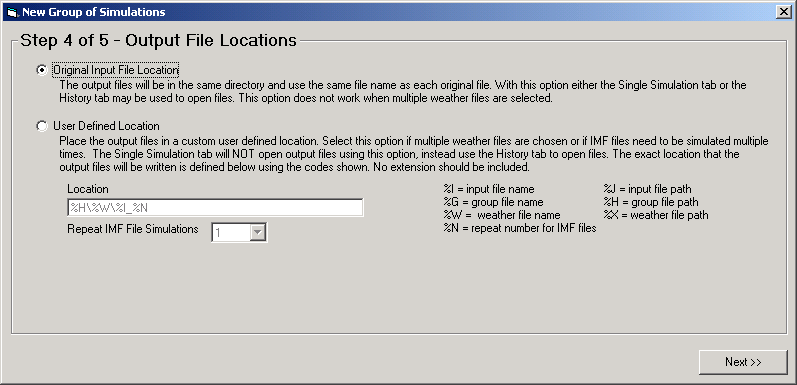
\includegraphics[width=0.9\textwidth, height=0.9\textheight, keepaspectratio=true]{media/image111.png}
\caption{Daylighting shelf DXF output. \protect \label{fig:daylighting-shelf-dxf-output.}}
\end{figure}

In EnergyPlus a daylighting shelf is simulated using a DaylightingDevice:Shelf object in combination with up to three other objects: a window, a heat transfer surface, and an attached shading surface.

The window must be divided into two window surfaces: an upper window and a lower window. The upper window interacts directly with the daylighting shelf object and is not allowed to have any shading control devices or frames or dividers. The lower window does not interact with the daylighting shelf object, but does receive shading from the outside shelf. There are no restrictions on the lower window.

The inside shelf is defined as a regular heat transfer surface in the zone. However, the surface must have the \emph{Outside Boundary Condition} field set to Surface with itself as the other zone surface. Shading and thermal mass effects are taken into account.

The outside shelf is defined as a \hyperref[shadingzonedetailed-000]{Shading:Zone:Detailed} object. The visible and solar absorptance of the outside material layer determines the reflectivity of the shelf.

\begin{callout}
  NOTE: Unlike a regular \hyperref[shadingzonedetailed-000]{Shading:Zone:Detailed} object, the vertices of the outside shelf surface must be ordered so that the outward normal vector points \emph{upward}, i.e. toward the upper window. This is necessary in order for the outside shelf to properly receive sunlight and shading from other surfaces. A mirror shading surface with the outward normal vector pointing in the opposite direction is automatically created by the program to shade the lower window.
\end{callout}

The inside shelf and outside shelf are both optional. However, if neither shelf is specified, the daylighting shelf object has no effect on the simulation.

\subsubsection{Inputs}\label{inputs-7-005}

\paragraph{Field: Name}\label{field-name-4-006}

The name of the daylighting shelf object.

\paragraph{Field: Window Name}\label{field-window-name-1}

Reference to a \hyperref[fenestrationsurfacedetailed]{FenestrationSurface:Detailed} object with \emph{Surface Type} WINDOW.

\paragraph{Field: Inside Shelf Name}\label{field-inside-shelf-name}

Reference to a \hyperref[buildingsurfacedetailed]{BuildingSurface:Detailed} object. This field is optional. If used, this surface must have OTHERZONESURFACE specified for the \emph{Outside Face Environment} field and the referenced other zone surface must be itself. The number of vertices of this surface object must be 4.

\paragraph{Field: Outside Shelf Name}\label{field-outside-shelf-name}

Reference to a \hyperref[shadingzonedetailed-000]{Shading:Zone:Detailed} object. This field is optional. If used, the number of vertices of this surface object must be 4.

\paragraph{Field: Outside Shelf Construction Name}\label{field-outside-shelf-construction-name}

Reference to a CONSTRUCTION object. This field is required if an outside shelf is specified. The visible and solar absorptance of the outside material layer determines the shelf reflectivity.

\paragraph{Field: View Factor To Outside Shelf}\label{field-view-factor-to-outside-shelf}

User defined value for the view factor from the window to the outside shelf. This field is optional. If not specified, an exact view factor is calculated for two perpendicular rectangles of the same width having a shared edge. If the given surfaces do not meet these geometric requirements, it is necessary to specify a value here.

\begin{callout}
  NOTE: It is up to the user to adjust the view factor to ground of the upper window to account for the part of the view blocked by the outside shelf. The calculated \emph{View Factor To Outside Shelf} is reported in the eio file for this purpose. For the typical case where the shelf is parallel to the ground and the upper window is perpendicular to the ground, the view factor to ground is simply: 0.5 -- \emph{View Factor To Outside Shelf}.
\end{callout}

\begin{lstlisting}
DaylightingDevice:Shelf,
    Shelf,  !- Name
    Daylit Upper Window,  !- Window Name
    Inside Shelf,  !- Inside Shelf Name
    Outside Shelf,  !- Outside Shelf Name
    Shelf Construction;  !- Outside Shelf Construction Name (required if outside shelf specified)
    ! 0.29;  !- View Factor To Outside Shelf (optional)

FenestrationSurface:Detailed,
    Daylit Upper Window,  !- Subsurface Name
    Window,  !- Surface Type
    Standard Window,  !- Construction Name
    Daylit South Wall,  !- Base Surface Name
    ,  !- Outside Face Environment
    0.211,  !- VF to Ground (user must adjust to account for view factor to outside shelf)
    ,  !- Window Shading Control (not allowed)
    ,  !- Frame/Divider Name (not allowed)
    1.0,  !- Multiplier (must be 1.0)
    4,  !- Number of Vertices
    1.0,  0.0,  2.8,
    1.0,  0.0,  2.0,
    4.0,  0.0,  2.0,
    4.0,  0.0,  2.8;

BuildingSurface:Detailed,
    Inside Shelf,  !- Surface Name
    Wall,  !- Surface Type
    Shelf Construction,  !- Construction Name
    Daylit Zone,  !- Zone Name
    OtherZoneSurface,  !- Exterior Conditions (must be OtherZoneSurface)
    Inside Shelf,  !- Target (must be itself)
    NoSun,  !- Solar Exposure
    NoWind,  !- Wind Exposure
    0.0,  !- VF to Ground
    4,  !- Number of Vertices
    1.0,  0.0,  2.0,
    4.0,  0.0,  2.0,
    4.0,  1.0,  2.0,
    1.0,  1.0,  2.0;

Shading:Zone:Detailed,
    Outside Shelf,  !- Surface Name
    Daylit South Wall,  !- Base Surface Name
    ,  !- Shading Transmittance Schedule (default is always opaque)
    4,  !- Number of Vertices
    1.0,  0.0,  2.0,  !- Outward normal vector must point up toward the upper window
    1.0, -1.0,  2.0,
    4.0, -1.0,  2.0,
    4.0,  0.0,  2.0;
\end{lstlisting}

\subsubsection{Outputs}\label{outputs-3-002}

The view factor to outside shelf calculation shows up in the .eio file along with the associated window and window view factors to sky and ground:

! \textless{}Shelf Details\textgreater{},Name,View Factor to Outside Shelf,Window Name,Window View Factor to Sky,Window View Factor to Ground

SHELF,0.29,DAYLIT UPPER WINDOW,0.50,0.21

This variable reports the calculated \emph{View Factor To Outside Shelf} so that the user can correctly adjust the view factor to ground of the upper window.

The usual window and surface variables are relevant for the upper window:

\begin{itemize}
\item
  Zone,Average,Surface Outside Face Sunlit Area {[}m2{]}
\item
  Zone,Average,Surface Outside Face Sunlit Fraction {[]}
\item
  Zone,Average,Surface Outside Face Incident Solar Radiation Rate per Area{[}W/m2{]}
\item
  Zone,Average,Surface Outside Face Incident Beam Solar Radiation Rate per Area{[}W/m2{]}
\item
  Zone,Average,Surface Outside Face Incident Sky Diffuse Solar Radiation Rate per Area{[}W/m2{]}
\item
  Zone,Average,Surface Outside Face Incident Ground Diffuse Solar Radiation Rate per Area{[}W/m2{]}
\item
  Zone,Average,Surface Outside Face Beam Solar Incident Angle Cosine Value{[]}
\item
  Zone,Average,Surface Window Transmitted Solar Radiation Rate {[}W{]}
\item
  Zone,Average,Surface Window Total Glazing Layers Absorbed Solar Radiation Rate {[}W{]}
\item
  Zone,Average,Surface Window Heat Gain Rate {[}W{]}
\item
  Zone,Average,Surface Window Heat Loss Rate {[}W{]}
\end{itemize}

The following surface variables are reported for the outside shelf surface, if specified:

\begin{itemize}
\item
  Zone,Average,Surface Outside Face Sunlit Area {[}m2{]}
\item
  Zone,Average,Surface Outside Face Sunlit Fraction {[]}
\item
  Zone,Average,Surface Outside Face Incident Solar Radiation Rate per Area{[}W/m2{]}
\item
  Zone,Average,Surface Outside Face Incident Beam Solar Radiation Rate per Area{[}W/m2{]}
\item
  Zone,Average,Surface Outside Face Incident Sky Diffuse Solar Radiation Rate per Area{[}W/m2{]}
\item
  Zone,Average,Surface Outside Face Incident Ground Diffuse Solar Radiation Rate per Area{[}W/m2{]}
\item
  Zone,Average,Surface Outside Face Beam Solar Incident Angle Cosine Value{[]}
\end{itemize}

\subsection{DaylightingDevice:LightWell}\label{daylightingdevicelightwell}

This object is used to model the impacts on daylighting of a ``light well'' that might be associated with exterior windows such as skylights.~ The light well model attenuates the light transmitted by the skylight. The attenuation is characterized by the \textbf{well efficiency}, which is the ratio of the amount of light leaving the well to the amount of light entering the well. The well efficiency varies from close to 1.0~ to close to zero if there is high attenuation. The well efficiency is used only in the EnergyPlus detailed daylighting calculation, where it multiplies the beam and diffuse light transmitted by the skylight. (The well efficiency is not used in calculating the solar gain through the skylight.)

The input object describes the light well using basic characteristics of the geometry along with the visible reflectance of the well's side walls.~ The following figure diagrams how the geometry is characterized.

\begin{figure}[hbtp] % fig 70
\centering
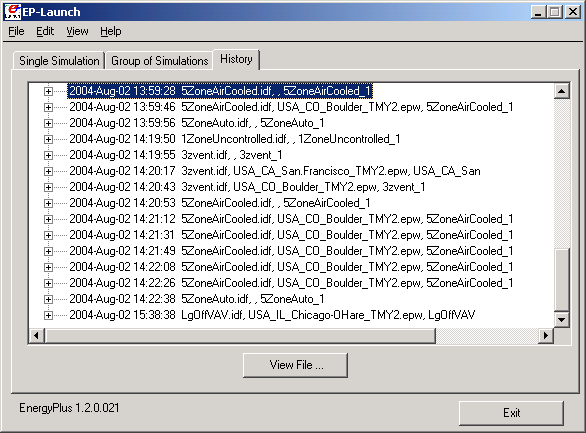
\includegraphics[width=0.9\textwidth, height=0.9\textheight, keepaspectratio=true]{media/image112.png}
\caption{Skylight with light well: (a) perspective view, (b) vertical section. If the bottom of the light well is a rectangle of side lengths c and d, as shown in (a), then the perimeter of the bottom of the well = 2(c+d) and the area = cd (see description of field names for the Light Well object). \protect \label{fig:skylight-with-light-well-a-perspective-view-b}}
\end{figure}

\subsubsection{Inputs}\label{inputs-8-004}

\paragraph{Field: Exterior Window Name}\label{field-exterior-window-name}

The name of the exterior window that this Light Well is associated with. Generally this is a skylight in a roof. However, light wells can be applied to an exterior window of any slope. Light wells can be assigned to both rectangular and triangular exterior windows, but they should not be assigned to interior windows. Note that the sides of the light well can be sloped and the bottom of the light well can be any shape, not~ just rectangular.

\paragraph{Field: Height of Well}\label{field-height-of-well}

The distance from the bottom of the skylight to the bottom of the well. If the skylight and well bottom are not coplanar, this is the distance from the center of the bottom of the skylight to center of the bottom of the well. See Figure~\ref{fig:skylight-with-light-well-a-perspective-view-b}.

\paragraph{Field: Perimeter of Bottom of Well}\label{field-perimeter-of-bottom-of-well}

The perimeter of the bottom opening of the well. See Figure~\ref{fig:skylight-with-light-well-a-perspective-view-b}.

\paragraph{Field: Area of Bottom of Well}\label{field-area-of-bottom-of-well}

The area of the bottom opening of the well. A warning will be issued if this area is less that the area of the skylight, including frame if present. See Figure~\ref{fig:skylight-with-light-well-a-perspective-view-b}.

\paragraph{Field: Visible Reflectance of Well Walls}\label{field-visible-reflectance-of-well-walls}

The visible reflectance of the side walls of the well. If the walls do not all have the same reflectance, an area-weighted average value can be used.~ This is the well-wall reflectance expressed as a fraction.

An IDF example:

\begin{lstlisting}
DaylightingDevice:LightWell,  ! The well is 60% reflecting, is 1.2m high and has a 2.5m x 5.5m bottom opening.
   Skylight-1, !- Name of Exterior Window that this Light Well Applies To
   1.2,        !- Height of Well(m)
   16.0,       !- Perimeter of Bottom of Well (m)
   13.75,      !- Area of Bottom of Well (m2)
   0.60;       !- Visible Reflectance of Well Walls
\end{lstlisting}

\subsection{Daylighting Modeling Options}\label{daylighting-modeling-options}

The following table shows what input objects/fields to use to model different daylighting options. It also gives the name of an example input, if available, that demonstrates the option.

% table 21
{\scriptsize
\begin{longtable}[c]{>{\raggedright}p{1.5in}>{\raggedright}p{3.0in}>{\raggedright}p{1.5in}}
\caption{Daylighting Modeling Options \label{table:daylighting-modeling-options}} \tabularnewline
\toprule
Option & Object/Field or Output Variable & Input File \tabularnewline
\midrule
\endfirsthead

\caption[]{Daylighting Modeling Options} \tabularnewline
\toprule
Option & Object/Field or Output Variable & Input File \tabularnewline
\midrule
\endhead

Allow a thermal zone to be daylit & Daylighting:Controls, Daylighting:ReferencePoint & PurchAirWithDaylighting.idf, DElight-Detailed-Comparison.idf \tabularnewline
Specify visible transmittance of the glazing & WindowMaterial:Glazing & PurchAirWithDaylighting.idf \tabularnewline
Specify the visible transmittance of a shading device & WindowMaterial:Shade, WindowMaterial:Screen or WindowMaterial:Blind & PurchAirWindowBlind.idf \tabularnewline
Use a shading device to control glare & WindowMaterial:Shade or WindowMaterial:Blind; WindowShadingControl* & PurchAirWindowBlind.idf \tabularnewline
Use electrochromic glazing to control glare & WindowShadingControl/Shading Type = SwitchableGlazing, Shading Control Type = On If High Glare, Glare Control Is Active = Yes* & PurchAirWithDaylighting.idf \tabularnewline
Adjust electrochromic glazing to just meet daylighting illuminance setpoint & WindowShadingControl/Shading Type = SwitchableGlazing, Shading Control Type = MeetDaylightIlluminanceSetpoint* & ~ \tabularnewline
Print an illuminance map & Daylighting:Illuminance Map* & ~ \tabularnewline
Control electric lighting response to daylight illuminance level & Daylighting:Controls/Lighting Control Type = Continuous, Stepped or Continuous/Off, plus other fields; or …. & PurchAirWithDaylighting.idf; DElight-Detailed-Comparison.idf \tabularnewline
Add a light shelf (with Daylighting:Controls) & DaylightingDevice:Shelf * & DaylightingDeviceShelf.idf \tabularnewline
Add a light shelf (with Daylighting:Controls) & Daylighting:Controls using DElight & DElightCFSLightShelf.idf \tabularnewline
Add a light pipe & DaylightingDevice:Tubular * & DaylightingDeviceTubular.idf \tabularnewline
Model a skylight having a light well & DaylightingDevice:LightWell * & ~ \tabularnewline
Model daylighting through double facade & See “Double Facades: Daylighting through Interior Windows”* & PurchAirWithDoubleFacadeDaylighting.idf \tabularnewline
Add diffusing (translucent) glass & WindowMaterial:Glazing/Solar Diffusing = Yes* & ~ \tabularnewline
Model complex fenestration & Daylighting:Controls using DElight & DElightCFSWindow.idf \tabularnewline
Get a radiosity-based interior light inter-reflection calculation & Daylighting:Controls using DElight & DElight-Detailed-Comparison.idf \tabularnewline
Find effect on daylighting of solar reflected from overhangs, neighboring buildings, etc. & Building/SolarDistribution uses “withReflections” option & ~ \tabularnewline
Find visible transmittance effect of dirt on window & WindowMaterial:Glazing/Dirt Correction Factor for Solar and Visible Transmittance* & ~ \tabularnewline
\bottomrule
\end{longtable}}

*Used only with \hyperref[daylightingcontrols-000]{Daylighting:Controls} with the SplitFlux Daylighting Method.

\begin{center}\rule{0.5\linewidth}{0.4pt}\end{center}

\protect\hyperlink{ux5fftnref1}{{[}1{]}} Formerly, only the exterior windows in a zone could provide daylight to that zone.
